%%%%%%%%%%%%%%%%%%%%%%%%%%%%%%%%%%%%%%%%%%%%%%%%%%%%%%%%%%%
\section{Online experiment}
\label{sec:expMethods}
%%%%%%%%%%%%%%%%%%%%%%%%%%%%%%%%%%%%%%%%%%%%%%%%%%%%%%%%%%%

% Experimental Methods
%%  Platform  
%%  Human Subjects
%%% recruited through social media
%%% IRB form  Protocol Number: 14-012E Protocol Title: Massive Manipulation: A n online user study on controlling large swarms of simple robot sApproval Date: 7/26/2013Expiration Date: 7/26/2014
%%% Costs  for experiment:  ??
%%% Instrumenting:
%%%% Google analytics, airbrake, etc.

%% wherein we describe our framework


We developed a flexible testing framework for online human-swarm interaction studies. Over 5,000 humans performed over 20,000 swarm-robotics experiments with this framework, logging almost 700 hours of experiments.
%There are two halves to our framework: the server backend and the client-side (in-browser) frontend. The server backend is responsible for tabulating results, serving webpages containing the frontend code, and for issuing unique identifiers to each experiment participant. The in-browser frontend is responsible for running an experiment---that is to say, accepting user input, updating the state of the robot swarm, and ultimately evaluating task completion.

%% wherein we outline the process that a user takes to participate in an experiment
%\subsection{Methods}

%\paragraph{Overview}

Our web server generates a unique identifier for each participant and sends it along with the landing page to the participant. 
%`This identifier is stored as a browser cookie and is attached to all results the participant generates. 
%The participant's browser prompts for confirmation of the terms-of-service and offers a menu of experiments.
%Once the participant selects an experiment, their browser makes a new request to the server to load the experiment's webpage. The server sends scaffold HTML describing the layout of the page and a script block containing the experiment. 
A script on the participant's browser runs the experiment and posts the experiment data to the server. 
%The participant is then given the option of playing again or trying a different experiment.

%A participant may view all of the experimental data we have gathered; this information is available as either a webpage, a JSON file, or a comma-separated value file.

%% wherein we preach the good word of Ruby and describe what the backend actually does
%\paragraph{Backend}

%The server backend is written in Ruby, using the Ruby-on-Rails (abbreviated \emph{Rails}) web development framework. Ruby is a dynamically-typed object-oriented scripting language with a strong emphasis on programmer ergonomics and metaprogramming support. It is well-suited for the creation of domain-specific languages for a variety of tasks, as exemplified by the Rails framework. Our backend serves assets (images, scripts, stylesheets, and so forth) to participants, selects the correct script to send to perform a particular experiment, and stores results.

%Each result is a database record containing the experiment name, the participant identifier, the duration of the experiment (time to completion), the number of robots involved, the detailed mode information of the experiment, and the user agent string of the browser running the experiment (which identifies the type of browser used by the participant). Rails automates the process of creating the relevant database-object bindings, and thus we spent little time creating or modifying the result records, allowing us to rapidly adapt the server to our needs--for example, adding tracking of the user agent and experiment mode both took less than five minutes of work on the server side.

%The experiment script file to be sent to the client is chosen with the uniform resource identifier (URI) for the experiment webpage; this done, the server will render the page requested by the participant and insert the script for the selected experiment. The Rails framework has a great deal of support for optimizing and compacting (\emph{minifying}) Javascript files.

%% wherein we decry the evils of javascript and explain why we use the browser
%\paragraph{Frontend}

%The client frontend which runs in the participant's browser is written in Javascript, a dynamically-typed prototype-oriented scripting language with some functional programming support. We make heavy use of the Underscore framework (a functional programming toolkit for Javascript) as well as the Javascript port of \href{http://box2d.org/}{Box2D} (a popular 2D physics engine with good support for rigid-body dynamics and fixed-timestep simulation). Our frontend also includes helper libraries for drawing robots, handling user input, and drawing graphs.

%Our framework uses a base task to represent the lifecycle of an experiment---{\bf  instantiation, simulation, evaluation}, and {\bf submission}. A particular experiment inherits from this prototype but overrides particular methods and adds its own variables for bookkeeping; this allows new or modified tasks to be created rapidly with minimal boilerplate code.

%\paragraph{Model}
%Our robots are disc-shaped, non-holonomic, and confined to the 2D plane.  The control input $u$ consists of a single bounded force vector that is applied to each robot, $|u|\le u_{max}$.  We include a linear ramp for this force value that starts at zero and increases to the maximum value in one second; this allows participants to do fine control of the robots by tapping the arrow keys.
%\begin{align}\label{eq:sysmodel}
%\dot{x}_i = u_x,  \qquad  \dot{y}_i = u_y.
%\end{align}

%During the {\bf instantiation} phase, an experiment sets up the web page elements with help text and other information, and creates the obstacles, particles, and workpieces that will be present during the experiment. It will also randomly select which mode to run in, if applicable.

%During the {\bf simulation} phase the robots are moved according to user input and given a chance to interact with each other and the environment. The current state of the experiment is then drawn.

%In the {\bf evaluation} phase the experiment's completion criteria are applied to the current experiment state: are the robots in the goal zone, are the workpieces in the correct place, and so forth. If the criteria are not met, the experiment repeats the simulation phase; if they are met, then the experiment proceeds to result submission.

%In the {\bf submission} phase experiment results are combined with other user data and submitted to the server for collection.
Anonymized human subject data was collected under IRB \#14357-01.

%As a means of encouraging user interaction, the results of other runs of the experiment are shown to the participant after submission along with merit badges displaying the number of experiments completed.

%% wherein we justify hours spent on facebook and hacker news  -- ha!  I'd like us to place links in the .tex for future reference
%Because our study involved recording data from human subjects, it required IRB approval before we could legally save user data (IRB \#14357-01).
%% IRB form  Protocol Number: 14-012E Protocol Title: Massive Manipulation: An online user study on controlling large swarms of simple robot sApproval Date: 7/26/2013Expiration Date: 7/26/2014
%Rice Federal-Wide Assurance Number: 00003890

%Subjects were recruited using a combination of social network effects and coordinated news posts. We asked our friends and colleagues to send links to our site to their friends via their preferred social networks, generally Twitter, Facebook, Google+, and through email. Additionally, we posted our site to several news aggregators in hopes that it would be seen and visited. Our first such posting was to \href{https://news.ycombinator.com/item?id=6277052}{Hacker News}, an aggregator run by the Y-Combinator accelerator company; this posting resulted in our first thousand trials. A second posting was made to Reddit, but did not seem to cause much traffic. A third posting was made to the  \href{http://robohub.org/researchers-use-single-joystick-to-control-swarm-of-rc-robots/}{Robohub.org} site. The traffic generated by these postings is shown in Fig.~\ref{fig:timePlayed}. 



%\begin{wrapfigure}{R}{0.5\textwidth}
%  \vspace{-20pt}
%  \begin{center}
%  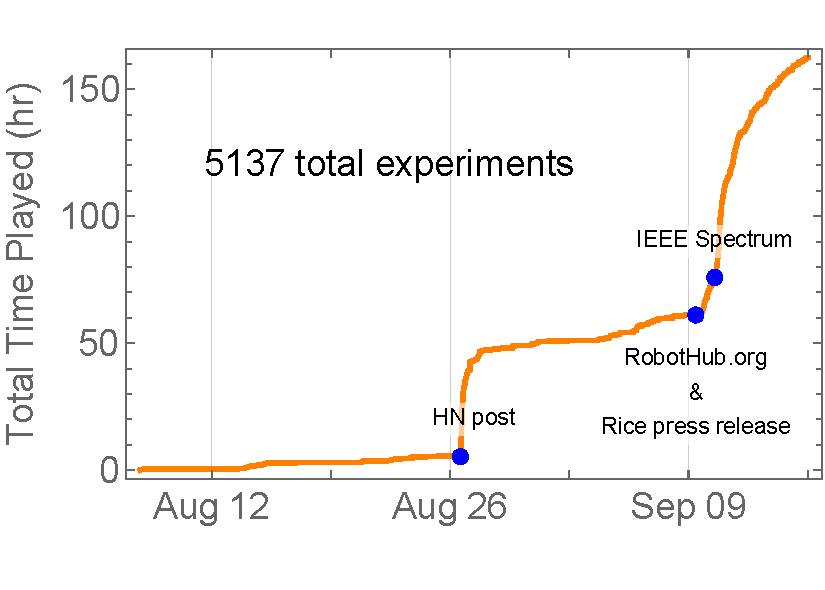
\includegraphics[width=0.5\textwidth]{timePlayed.pdf}
%  \end{center}
%  \vspace{-3em}
%\caption{
%\label{fig:timePlayed}
%Cumulative time played for completed tests during first two months.
%}
%\end{wrapfigure}

%\begin{figure}
%\centering
%\begin{overpic}[width = .5\columnwidth]{timePlayed.pdf}\end{overpic}
%\vspace{-2em}
%\caption{
%\label{fig:timePlayed}
%Cumulative time played for completed tests during first two months.
%}
%%\vspace{-2em}
%\end{figure}


%Concurrently, we contacted our university's  \href{http://news.rice.edu/contact-us/}{\emph{News and Media Relations Team}}. They sent a writer and photographer to our lab, worked with us to draft a \href{http://news.rice.edu/2013/09/09/a-swarm-on-every-desktop-robotics-experts-learn-from-public/ }{press release}, and publicized with news outlets and alumni. Most universities have a media team, and this is a valuable no-cost resource to gain publicity.
 
%% wherein we show just how cheap we are 
%\subsubsection{Experimental costs}

%We've spent approximately one hundred dollars USD provisioning and running this experiment. Hosting is provided by \href{Heroku.com}{Heroku}, using a single web instance costing around \$40/month, with additional monitoring services bringing that up to \$50/month. In the event of increased demand/participant traffic, we can provision another server to take up the load.
%We purchased our domain name from \href{Namecheap.com}{Namecheap.com} for \$11.66 a year, giving our site a short, easy to pronounce handle.
%SwarmControl.net %16 char
%SwarmControl.herokuapp.com %26 char

%As mobile traffic becomes more prominent and overtakes the volume of internet access from desktop computers & laptops, shorter domain names will become increasingly more important and more desirable.  The likelihood of a typo on a mobile device is increased and that  can be hedged by having a shorter domain name which requires less typing and fewer characters to enter. - See more at: http://www.mediaoptions.com/domain-names/short-is-sweet-the-value-of-short-domain-names.html#sthash.AJNqlXhB.dpuf

%Given the large number of experiment sessions run (over 11,000 at the time of this writing), we see a per-experiment cost of less than three cents.

%% wherein we describe how we monitor the progress of the experimental setup
%\subsubsection{Instrumentation}

%When conducting an online experiment, it is helpful to gather data about both the experiment infrastructure and the participants. For the backend, we use a service called Airbrake to monitor the Rails server, getting emails in the events of any errors occurring or suspicious activity. We also use another service called New Relic to provide monitoring and analytics on the server traffic, giving coarse statistics about site visitation, page load time, and other indicators of how our backend is performing.

%For the frontend, we use Google Analytics to track user behavior. This tool allows us to see country of origin for users, time spent on the site, relative percent of people who look past the landing page (bounce rate), and user agent information (type of browser, type of device, etc.).
